\lab{QR 2: Least Squares and Computing Eigenvalues}{Least Squares and Computing Eigenvalues}
\label{lab:qr-applications}
\objective{Because of its numerical stability and convenient structure, the QR decomposition is the basis of many important and practical algorithms.
In this lab, we introduce linear least squares problems, tools in Python for computing least squares solutions, and two fundamental eigenvalue algorithms.
\\ \indent As in the previous lab, we restrict ourselves to real matrices and therefore use the transpose in place of the Hermitian conjugate.}

\section*{Least Squares} % ====================================================

A linear system $A\x = \b$ is \emph{overdetermined} if it has more equations than unknowns.
In this situation, there is no true solution, and $\x$ can only be approximated.

The \emph{least squares solution} of $A\x = \b$, denoted as $\widehat{\x}$, is the ``closest'' vector to a solution, meaning it minimizes the quantity $\|A\widehat{\x} - \b\|_2$.
% \footnote{The choice of the 2-norm is significant.}
In other words, $\widehat{\x}$ is the vector such that $A\widehat{\x}$ is projection of $\b$ onto the range of $A$, and can be calculated by solving the \emph{normal equation}:%
\footnote{See Volume 1 Chapter 3 for a formal derivation of the normal equation.}
\[A\trp A\widehat{\x} = A\trp \b\]

If $A$ is full rank, which it usually is in applications, its QR decomposition provides an efficient way to solve the normal equation.
Let $A = \widehat{Q}\widehat{R}$ be the reduced QR decomposition of $A$, so $\widehat{Q}$ is $m \times n$ with orthonormal columns and $\widehat{R}$ is $n \times n$, invertible, and upper triangular.
Since $\widehat{Q}\trp \widehat{Q} = I$, and since $\widehat{R}\trp$ is invertible, the normal equation can be reduced as follows (we omit the hats on $\widehat{Q}$ and $\widehat{R}$ for clarity):
%
\begin{align}
\nonumber
A\trp A\widehat{\x} &= A\trp \b \\ \nonumber
(Q R)\trp Q R  \widehat{\x}
&= (Q R)\trp \b \\ \nonumber
 R\trp Q\trp Q R  \widehat{\x}
&=  R\trp Q\trp \b \\ \nonumber
 R\trp R \widehat{\x}
&=  R\trp Q\trp \b \\
 R \widehat{\x}
&= Q\trp \b \label{eq:normal-equation-via-qr}
\end{align}

Thus $\widehat{\x}$ is the least squares solution to $A\x=\b$ if and only if $\widehat{R}\widehat{\x} = \widehat{Q}\trp\b.$
Since $\widehat{R}$ is upper triangular, this equation can be solved quickly with back substitution.

\begin{problem} % Solve the normal equations with QR.
Write a function that accepts an $m \times n$ matrix $A$ of rank $n$ and a vector $\b$ of length $n$.
Use the QR decomposition and Equation \ref{eq:normal-equation-via-qr} to solve the normal equation corresponding to $A\x = \b$.

You may use either SciPy's QR routine or one of your own routines from the previous lab.
In addition, you may use \li{la.solve_triangular()}, SciPy's optimized routine for solving triangular systems.

\label{prob:lstsq-via-qr}
\end{problem}

\subsection*{Fitting a Line} % ------------------------------------------------

The least squares solution can be used to find the best-fit curve of a chosen type to a set of points.
Consider the problem of finding the line $y = ax + b$ that best fits a set of $m$ points $\{(x_k, y_k)\}_{k=1}^m$.
Ideally, we seek $a$ and $b$ such that $y_k = ax_k + b$ for all $k$.
The following linear system simultaneously represents all of these equations.
%
\begin{equation}
A\x =
\left[\begin{array}{cc}
x_1 & 1 \\
x_2 & 1 \\
x_3 & 1 \\
\vdots & \vdots \\
x_m & 1
\end{array}\right]
\left[\begin{array}{c} a \\ b \end{array}\right]
=
\left[\begin{array}{c} y_1 \\ y_2 \\ y_3 \\ \vdots \\ y_m \end{array}\right]
= \b
\label{eq:linear-least-squares}
\end{equation}
%
Note that $A$ has full column rank as long as not all of the $x_k$ values are the same.

Because this system has two unknowns, it is guaranteed to have a solution if it has two or fewer equations.
However, if there are more that two data points, the system is overdetermined if any set of three points are not collinear.
We therefore seek a least squares solution, which in this case means finding the slope $\widehat{a}$ and $y$-intercept $\widehat{b}$ such that the line $y = \widehat{a}x+\widehat{b}$ best fits the data.

Figure \ref{fig:line-fit-example} is a typical example of this idea where $\widehat{a} \approx \frac{1}{2}$ and $\widehat{b} \approx -3$.

\begin{figure}[H] % Linear regression example (without code).
    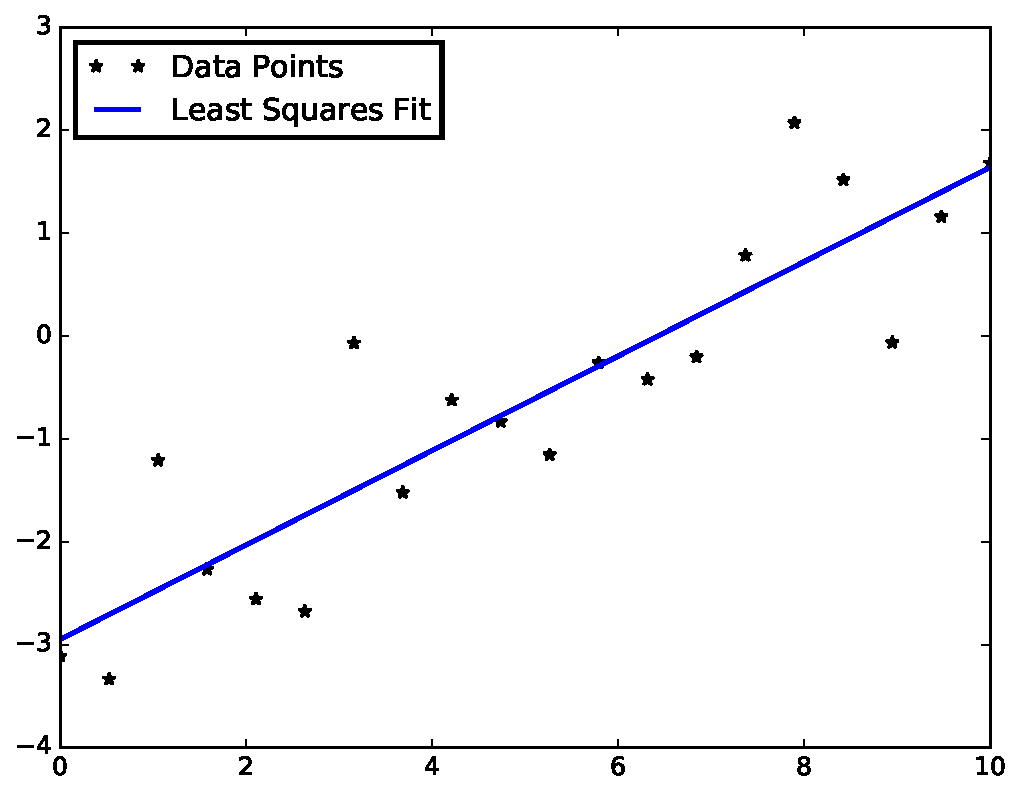
\includegraphics[width=.59\textwidth]{figures/line_fit_example.pdf}
    \caption{}
    \label{fig:line-fit-example}
\end{figure}

% TODO: Consider replacing this data set with something with less variance.
% This data set is also used in the Data Visualization lab.
\begin{problem} % Linear regression of height vs weight.
The file \texttt{MLB.npy} contains measurements from over 1,000 recent Major League Baseball players, compiled by UCLA.\footnote{See \url{http://wiki.stat.ucla.edu/socr/index.php/SOCR_Data_MLB_HeightsWeights}.}
Each row in the array represents a different player; the columns are the player's height (in inches), weight (in pounds), and age (in years), in that order.

Find the least squares line that relates the height of the players to their weight (i.e., let height be the $x$ values and weight be the $y$ values).
%
\begin{enumerate}
    \item Construct the matrix $A$ and the vector $\b$ described by Equation \ref{eq:linear-least-squares}.\\
    (Hint: the functions \li{np.vstack()}, \li{np.column_stack()}, and/or \li{np.ones()} may be helpful.)
    \item Use your function from Problem \ref{prob:lstsq-via-qr} to find the least squares solution.
    \item Plot the data points as a scatter plot.
    \item Plot the least squares line with the scatter plot.\\
    (Hint: Make a new domain of $x$ values with \li{np.linspace()}, and use this domain to calculate $y = \widehat{a}x + \widehat{b}$.)
\end{enumerate}
\end{problem}

\begin{info} % scipy.stats.linregress().
The least squares problem of fitting a line to a set of points is often called \emph{linear regression}, and the resulting line is called the \emph{linear regression line}.
SciPy's specialized tool for linear regression is \li{scipy.stats.linregress()}.
This function takes in an array of $x$-coordinates and a corresponding array of $y$-coordinates, and returns the slope and intercept of the regression line, along with a few other statistical measurements.

For example, the following code produces Figure \ref{fig:line-fit-example}.

\begin{lstlisting}
>>> import numpy as np
>>> from scipy.stats import linregress

# Generate some random data close to the line y = .5x - 3.
>>> x = np.linspace(0, 10, 20)
>>> y = .5*x - 3 + np.random.randn(20)

# Use linregress() to calculate m and b, as well as the correlation
# coefficient, p-value, and standard error. See the documentation for
# details on each of these extra return values.
>>> a, b, rvalue, pvalue, stderr = linregress(x, y)

>>> plt.plot(x, y, 'k*', label="Data Points")
>>> plt.plot(x, a*x + b, 'b-', lw=2, label="Least Squares Fit")
>>> plt.legend(loc="upper left")
>>> plt.show()
\end{lstlisting}
\end{info}

\subsection*{Fitting a Polynomial} % ------------------------------------------

Least squares can also be used to fit a set of data to the best-fit polynomial of a specified degree.
Let $\{(x_k, y_k)\}_{k=1}^m$ be the set of $m$ data points in question.
The general form for a polynomial of degree $n$ is as follows:
\[
p_n(x) = c_n x^n + c_{n-1} x^{n-1} + \cdots + c_2 x^2 + c_1 x + c_0
\]
Note that the polynomial is uniquely determined by its $n+1$ coefficients $\{c_k\}_{k=0}^n$.
Ideally, then, we seek the set of coefficients $\{c_k\}_{k=0}^n$ such that
\[
y_k = c_n x_k^n + c_{n-1} x_k^{n-1} + \cdots + c_2 x_k^2 + c_1 x_k + c_0
\]
for all values of $k$.
These $m$ linear equations yield the following linear system:
\begin{equation}
A\x =
\left[\begin{array}{cccccc}
x_1^n & x_1^{n-1} & \cdots & x_1^2 & x_1 & 1 \\
x_2^n & x_2^{n-1} & \cdots & x_2^2 & x_2 & 1 \\
x_3^n & x_3^{n-1} & \cdots & x_3^2 & x_3 & 1 \\
\vdots & \vdots & & \vdots & \vdots & \vdots \\
x_m^n & x_m^{n-1} & \cdots & x_m^2 & x_m & 1 \\
\end{array}\right]
\left[\begin{array}{c}
c_n \\ c_{n-1} \\ \vdots \\ c_2 \\ c_1 \\ c_0
\end{array}\right]
=
\left[\begin{array}{c} y_1 \\ y_2 \\ y_3 \\ \vdots \\ y_m \end{array}\right]
= \b
\label{eq:polynomial-least-squares}
\end{equation}
%
If $m > n+1$ this system is overdetermined, requiring a least squares solution.

\subsubsection*{Working with Polynomials in NumPy} % - - - - - - - - - - - - -

The $m \times (n+1)$ matrix $A$ of Equation \ref{eq:polynomial-least-squares} is called a \emph{Vandermonde matrix}.%
\footnote{Vandermonde matrices have many special properties and are useful for many applications, including polynomial interpolation and discrete Fourier analysis.}
% a matrix with entries $a_{ij} = x_i^{n-j+1}$.
NumPy's \li{np.vander()} is a convenient tool for quickly constructing a Vandermonde matrix, given the values $\{x_k\}_{k=1}^m$ and the number of desired columns.

\begin{lstlisting}
>>> print(np.vander([2, 3, 5], 2))
[[2 1]
 [3 1]
 [5 1]]

>>> print(np.vander([2, 3, 5, 4], 3))
[[ 4  2  1]
 [ 9  3  1]
 [25  5  1]
 [16  4  1]]
\end{lstlisting}

NumPy also has powerful tools for working efficiently with polynomials.
The class \li{np.poly1d} represents a 1-dimensional polynomial.
Instances of this class are callable like a function.%
\footnote{Class instances can be made callable by implementing the \li{__call__()} magic method.}
The constructor accepts the polynomial's coefficients, from largest degree to smallest.

Table \ref{table:numpy-poly1d} lists the attributes and methods of the \li{np.poly1d} class.
See \url{http://docs.scipy.org/doc/numpy/reference/routines.polynomials.html} for a list of NumPy's polynomial routines.

\begin{table}[H]
\begin{tabular}{r|l}
    Attribute & Description \\
    \hline
    coeffs & The $n+1$ coefficients, from greatest degree to least. \\
    order & The polynomial degree ($n$). \\
    roots & The $n-1$ roots. \\
    \\
    Method & Returns \\
    \hline
    deriv() & The coefficients of the polynomial after being differentiated. \\
    integ() & The coefficients of the polynomial after being integrated (with $c_0 = 0$).
\end{tabular}
\caption{Attributes and methods of the \li{np.poly1d} class.}
\label{table:numpy-poly1d}
\end{table}
%
\begin{lstlisting}
# Create a callable object for the polynomial f(x) = (x-1)(x-2) = x^2 - 3x + 2.
>>> f = np.poly1d([1, -3, 2])
>>> print(f)
   2
1 x - 3 x + 2

# Evaluate f(x) for several values of x in a single function call.
>>> f([1, 2, 3, 4])
array([0, 0, 2, 6])

# Evaluate f(x) at 1, 2, 3, and 4 without creating f(x) explicitly.
>>> np.polyval([1, -3, 2], [1, 2, 3, 4])
array([0, 0, 2, 6])
\end{lstlisting}

\begin{problem} % Polynomial fitting.
The file \texttt{polynomial.npy} contains an array of $20$ $(x,y)$ coordinate pairs.
Each row of the array is a different coordinate pair, with $x$ values in the first column and $y$ values in the second column.

Write a function that uses Equation \ref{eq:polynomial-least-squares} to calculate the polynomials of degree $3$, $5$, $7$, and $19$ that best fit the data.
Plot the original data points and each least squares polynomial together in individual subplots.\\
(Hint: set the window limits to be the same on each subplot to get an accurate picture of what's happening with the degree $19$ polynomial).

Instead of using Problem \ref{prob:lstsq-via-qr} to solve the normal equation, you may use \li{scipy.linalg.lstsq()}, demonstrated below.
% Compare your results to \li{np.polyfit()}.
% This function receives arrays of $x$ and $y$ values and an integer for the degree, and returns the coefficients of the best-fit polynomial of that degree.

\begin{lstlisting}
>>> from scipy import linalg as la

# Define A and b appropriately.

# Solve the normal equation using SciPy's least squares routine.
# The least squares solution is the first of four return values.
>>> x = la.lstsq(A, b)[0]
\end{lstlisting}

Compare your results to \li{np.polyfit()}.
This function receives an array of $x$ values, an array of $y$ values, and an integer for the polynomial degree, and returns the coefficients of the best-fit polynomial of that degree.

\label{prob:polynomial-least-squares}
\end{problem}

\begin{warn} % Overfitting
Problem \ref{prob:polynomial-least-squares} demonstrates that having more parameters in a least squares model is not always better.
The polynomial of degree 19 actually \emph{interpolates} the data set, meaning that $p_{19}(x_k) = y_k$ exactly for each $k$, because there are enough unknowns that the system is no longer overdetermined.

Choosing to have too many unknowns in a fitting problem is (fittingly) called \emph{overfitting}, and is an important issue to avoid in any statistical model.
\end{warn}

\subsection*{Fitting a Circle} % ----------------------------------------------

Suppose the set of $m$ points $\{(x_k, y_k)\}_{k=1}^m$ are arranged in a nearly circular pattern.
The general equation of a circle with radius $r$ and center $(c_1, c_2)$ is as follows:
\begin{equation}
(x-c_1)^2 + (y-c_2)^2 = r^2.
\label{eq:standard-circle}
\end{equation}

The circle is uniquely determined  by $r$, $c_1$, and $c_2$, so these are the parameters that should be solved for in a least squares formulation of the problem.
However, Equation \ref{eq:standard-circle} is not linear in any of these variables.
%
\begin{align}
\nonumber (x - c_1)^2 + (y - c_2)^2 &= r^2 \\
\nonumber x^2 - 2c_1 x + c_1^2 + y^2 - 2c_2y + c_2^2 &= r^2 \\
x^2 + y^2 & = 2c_1 x + 2c_2 y + \textcolor{red}{r^2 - c_1^2 - c_2^2}
\label{eq:circle-expanded}
\end{align}

The quadratic terms $x^2$ and $y^2$ are acceptable because the points $\{(x_k, y_k)\}_{k=1}^m$ are given.
To eliminate the nonlinear terms in the unknown parameters $r$, $c_1$, and $c_2$, define a new variable $c_3 = r^2 - c_1^2 - c_2^2$.
Then for each point $(x_k, y_k)$, Equation \ref{eq:circle-expanded} becomes the following:
\[2c_1x_k + 2c_2y_k + \textcolor{red}{c_3} = x_k^2 + y_k^2\]
These $m$ equations are linear in $c_1$, $c_2$, and $c_3$, and can be written as a linear system.

\begin{equation}
\left[\begin{array}{ccc}
2 x_1 & 2 y_1 & 1 \\
2 x_2 & 2 y_2 & 1 \\
\vdots & \vdots & \vdots \\
2 x_m & 2 y_m & 1
\end{array}\right]
\left[\begin{array}{c} c_1 \\ c_2 \\ c_3 \end{array}\right]
=
\left[\begin{array}{c}
x_1^2 + y_1^2 \\
x_2^2 + y_2^2 \\
\vdots \\
x_m^2 + y_m^2
\end{array}\right]
\label{eq:circle-least-squares}
\end{equation}

After solving for the least squares solution, $r$ can be recovered with the relation $r = \sqrt{c_1^2 + c_2^2 + c_3}$.
Finally, plotting a circle is best done with polar coordinates.
Using the same variables as before, the circle can be represented in polar equations with the following equations:
\begin{align*}
x = r\cos(\theta) + c_1 && y = r\sin(\theta) + c_2,
\end{align*}
where $\theta \in [0, 2\pi]$.

\begin{lstlisting}
# Load some data and construct the matrix A and the vector b.
>>> xk, yk = np.load("circle.npy").T
>>> A = np.column_stack((2*x, 2*y, np.ones_like(x)))
>>> b = xk**2 + yk**2

# Calculate the least squares solution and calculate the radius.
>>> c1, c2, c3 = la.lstsq(A, b)[0]
>>> r = np.sqrt(c1**2 + c2**2 + c3)

# Plot the circle using polar coordinates.
>>> theta = np.linspace(0, 2*np.pi, 200)
>>> x = r*np.cos(theta) + c1
>>> y = r*np.sin(theta) + c2
>>> plt.plot(x, y, '-', lw=2)
>>> plt.plot(xk, yk, 'k*')
>>> plt.axis("equal")
\end{lstlisting}

\begin{figure}[H]
    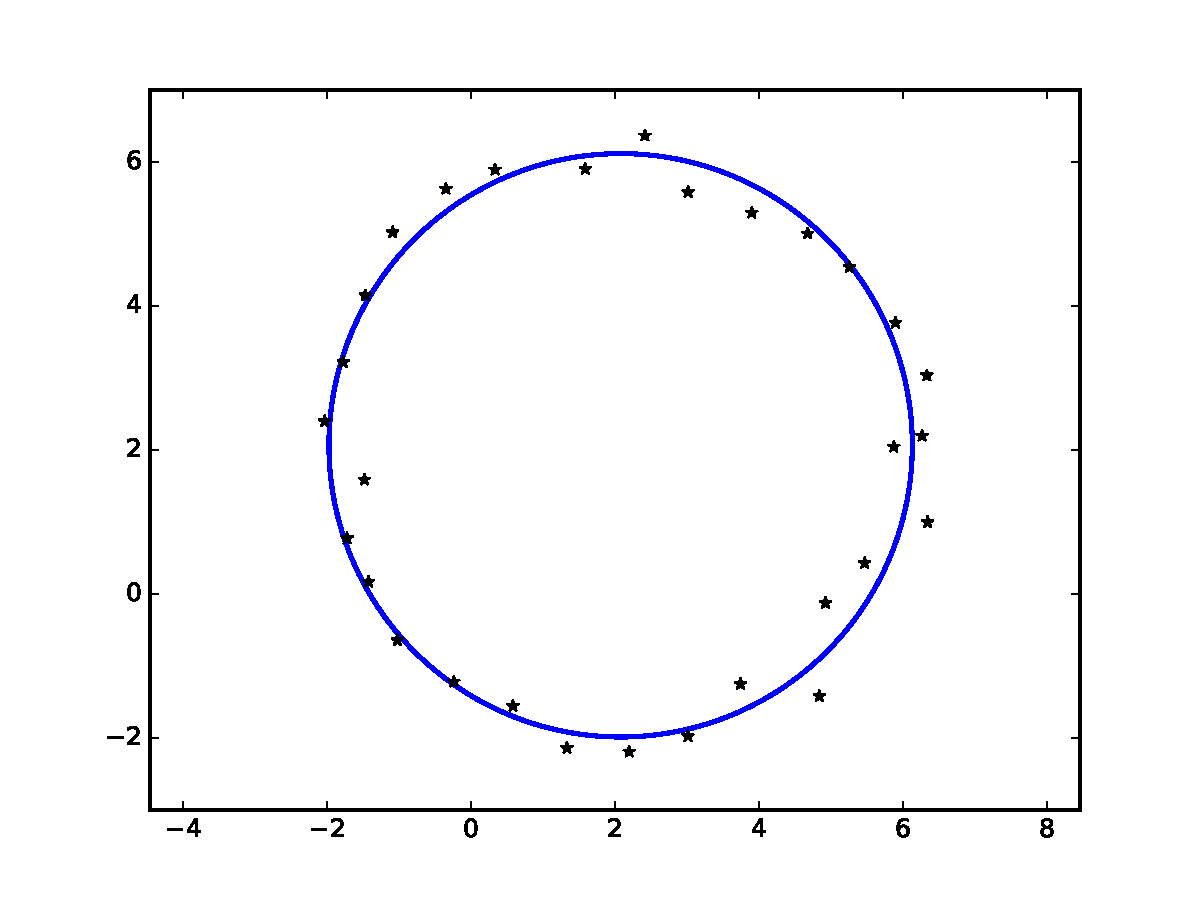
\includegraphics[width=.55\textwidth]{figures/circle_fit_example.pdf}
\end{figure}

\begin{problem}
The general equation for an ellipse is \[ax^2 + bx + cxy + dy + ey^2 = 1.\]
Write a function that calculates the parameters for the ellipse that best fits the data in the file \texttt{ellipse.npy}.
Plot the original data points and the ellipse together, using the following function to plot the ellipse.

\begin{lstlisting}
def plot_ellipse(a, b, c, d, e):
    """Plot an ellipse of the form ax^2 + bx + cxy + dy + ey^2 = 1."""
    theta = np.linspace(0, 2*np.pi, 200)
    cos_t, sin_t = np.cos(theta), np.sin(theta)
    A = a*(cos_t**2) + c*cos_t*sin_t + e*(sin_t**2)
    B = b*cos_t + d*sin_t
    r = (-B + np.sqrt(B**2 + 4*A))/(2*A)

    plt.plot(r*cos_t, r*sin_t, lw=2)
    plt.gca().set_aspect("equal", "datalim")
\end{lstlisting}
\end{problem}

\section*{Computing Eigenvalues} % ============================================

The eigenvalues of an $n \times n$ matrix $A$ are the roots of its characteristic polynomial $\det(A - \lambda I)$.
Thus, finding the eigenvalues of $A$ amounts to computing the roots of a polynomial of degree $n$.
However, for $n \ge 5$, it is provably impossible to find an algebraic closed-form solution to this problem.%
\footnote{This result, called \emph{Abel's impossibility theorem}, was first proven by Niels Heinrik Abel in 1824.}
In addition, numerically computing the roots of a polynomial is a famously ill-conditioned problem, meaning that small changes in the coefficients of the polynomial (brought about by small changes in the entries of $A$) may yield wildly different results.
Instead, eigenvalues must be computed with iterative methods.

\subsection*{The Power Method} % ----------------------------------------------

The \emph{dominant eigenvalue} of the $n \times n$ matrix $A$ is the unique eigenvalue of greatest magnitude, if such an eigenvalue exists.
The \emph{power method} iteratively computes the dominant eigenvalue of $A$ and its corresponding eigenvector.

Begin by choosing a vector $\x_0$ such that $\|\x_0\|=1$, and define the following:
\[\x_{k+1}=\frac{A\x_k}{\|A\x_k\|}\]
If $A$ has a dominant eigenvalue $\lambda$, and if the projection of $\x_0$ onto the subspace spanned by the eigenvectors corresponding to $\lambda$ is nonzero, then the sequence of vectors $\{\x_k\}_{k=0}^\infty$ converges
% \footnote{Reference proof in the text}
to an eigenvector $\x$ of $A$ corresponding to $\lambda$.

Since $\x$ is an eigenvector of $A$, $A\x = \lambda \x$.
Left multiplying by $\x\trp$ on each side gives $\x\trp A\x = \lambda \x\trp\x$, and hence $\lambda = \frac{\x\trp A\x}{\x\trp\x}$.
This ratio is called the \emph{Rayleigh quotient}.
However, since each $\x_k$ is normalized, $\x\trp\x = \|\x\|^2 = 1$, so $\lambda = \x\trp A\x$.

The entire algorithm is summarized below.

\begin{algorithm}[H] % The Power Method
\begin{algorithmic}[1]
\Procedure{Power Method}{$A$}
    \State $m, n \gets \shape{A}$
        \Comment{Store the dimensions of $A$.}
    \State $\x_0 \gets \text{random}(n)$
        \Comment{A random vector of length $n$}
    \State $\x_0 \gets \x_0/\|\x_0\|$
        \Comment{Normalize $\x_0$}
    \For{$k = 1,\ 2,\ \ldots,\ N-1$}
        \label{step:power-method-stopping-criterion}
        \State $\x_{k+1} \gets A\x_k$
        \State $\x_{k+1} \gets \x_{k+1}/\|\x_{k+1}\|$
    \EndFor
    \State \pseudoli{return} $\x_N\trp A \x_N,\ \x_N$
\EndProcedure
\end{algorithmic}
\caption{}
\label{Alg:power-method}
\end{algorithm}

The power method is limited by a few assumptions.
First, not all square matrices $A$ have a dominant eigenvalue.
For testing purposes, the Perron-Frobenius theorem%
\footnote{See Chapter ?? of the Volume I text for a careful proof of the theorem.}
guarantees that if all entries of $A$ are positive, then $A$ has a dominant eigenvalue.
Second, there is no way to choose an $\x_0$ that is guaranteed to have a nonzero projection onto the span of the eigenvectors corresponding to $\lambda$.
However, a random $\x_0$ will almost surely satisfy this condition.

% TODO: Footnote about the proof of the power method?

\begin{problem} % Implement the power method.
Write a function that accepts an $n \times n$ matrix $A$, a float \li{tol}, and a maximum number of iterations $N$.
Use Algorithm \ref{Alg:power-method} to compute the dominant eigenvalue of $A$ and a corresponding eigenvector.

Continue the loop in step \ref{step:power-method-stopping-criterion} until either $\|\x_{k+1} - \x_k\|$ is less than the tolerance \li{tol}, or until iterating the maximum number of times $N$.

Test your function on square matrices with all positive entries, verifying that $A\x = \lambda\x$.
Use SciPy's eigenvalue solver, \li{scipy.linalg.eig()}, to compute all of the eigenvalues and corresponding eigenvectors of $A$ and check that $\lambda$ is the dominant eigenvalue of $A$.

\begin{lstlisting}
# Construct a random matrix with positive entries.
>>> A = np.random.random((10,10))

# Compute the eigenvalues and eigenvectors of A via SciPy.
>>> eigs, vecs = la.eig(A)

# Get the dominant eigenvalue and eigenvector of A.
# The eigenvector of the kth eigenvalue is the kth column of 'vecs'.
>>> loc = np.argmax(eigs)
>>> lamb, x = eigs[loc], vecs[:,loc]

# Verify that Ax = lambda x.
>>> np.allclose(A.dot(x), lamb*x)
True
\end{lstlisting}
\end{problem}

% TODO: A note about the convergence of the power method?

\begin{comment} % TODO: eliminate
The matrix $A$ can be written in Jordan Conical form $A=VJV^{-1}$ where $V$ is the matrix of the generalized eigenspaces.
But the first column is is the eigenvector corresponding to largest eigenvalue and $J$ is an upper triangular matrix of eigenvalues and ones.
Note that $A^k=VJ^kV^{-1}$
The limit as $k \rightarrow \infty$ of $(\frac{1}{\lambda_1}J)^k$ is a matrix of all zeros except for a one in the upper right hand corner.
So $(\frac{A}{\norm{A}})^k \approx VJ^kV^{-1}$, and the largest eigenvalue dominates.
\end{comment}

\subsection*{The QR Algorithm} % ----------------------------------------------

An obvious shortcoming of the power method is that it only computes the largest eigenvalue and a corresponding eigenvector.
The QR algorithm, on the other hand, attempts to find all eigenvalues of $A$.

Let $A_0 = A$, and for arbitrary $k$ let $Q_kR_k$ be the QR decomposition of $A_k$.
Since $A$ is square, so are $Q_k$ and $R_k$, so they can be recombined in reverse order.
\[A_{k+1}=R_kQ_k\]
This recursive definition establishes an important relation.
\[Q_k^{-1}A_kQ_k = Q_k^{-1}(Q_kR_k)Q_k = (Q_k^{-1}Q_k)(R_kQ_k) = A_{k+1}\]
Thus $A_k$ is similar to $A_{k+1}$, and similar matrices have the same eigenvalues.
% Furthermore, since each of the $Q_k$ are orthonormal, the computation is numerically stable.
The series of matrices $\{A_k\}_{k=0}^\infty$ converges to the following block matrix.
\[
S =
\left[\begin{array}{cccc}
S_1    & *      & \cdots & *      \\
\0     & S_2    & \ddots & \vdots \\
\vdots & \ddots & \ddots & *      \\
\0     & \cdots &     \0 & S_m
\end{array}\right]
\]

Each $S_i$ is either a $1\times1$ or $2\times2$ matrix.%
\footnote{If all of the $S_i$ are $1\times1$ matrices, then the upper triangular $S$ is called the \emph{Schur form} of $A$.
If some of the $S_i$ are $2\times2$ matrices, then $S$ is called the \emph{real Schur form} of $A$.}
Since $S$ is block upper triangular, its eigenvalues are the eigenvalues of its diagonal $S_i$ blocks.
Then because $A$ is similar to each $A_k$, those eigenvalues of $S$ are the eigenvalues of $A$.

% Second, each iteration of the algorithm transfers some of the ``mass'' from the lower to the upper triangle.
% This is what makes $A_0, A_1, A_2, \ldots$ converge to a matrix $S$ which has the described form.

When $A$ has real entries but complex eigenvalues, $2 \times 2$ $S_i$ blocks appear in $S$.
Finding eigenvalues of a $2 \times 2$ matrix is equivalent to finding the roots of a 2nd degree polynomial.
%
\begin{align}
\nonumber \det(S_i - \lambda I) =
\left|\begin{array}{cc}
a - \lambda & b           \\
c           & d - \lambda
\end{array}\right|
&= (a - \lambda)(d - \lambda) - bc \\
&= \lambda^2 - ad\lambda + (ad - bc) \label{eq:qr-algorithm-roots}
\end{align}

The quadratic equation is the closed-form algebraic solution for the roots of Equation \ref{eq:qr-algorithm-roots}.
Using $A = 1$, $B = -ad$, and $C = ad - bc$,
\[\lambda = \frac{-B \pm \sqrt{B^2 - 4AC}}{2A}.\]

\subsubsection*{Hessenberg Preconditioning} % - - - - - - - - - - - - - - - - -

The QR algorithm works more accurately and efficiently on matrices that are in upper Hessenberg form, as upper Hessenberg matrices are already close to triangular.
Furthermore, if $H = QR$ is the QR decomposition of upper Hessenberg $H$ then $RQ$ is also upper Hessenberg.
Putting a matrix in upper Hessenberg form before applying the QR algorithm is called \emph{Hessenberg preconditioning}.

% Second, an iteration of the QR algorithm can be computed in $\mathcal{O}(n^2)$ time on an upper Hessenberg matrix, as opposed to $\mathcal{O}(n^3)$ time on a regular matrix.
% This is because so many entries of an upper Hessenberg matrix are 0.
% If we apply the QR algorithm to an upper Hessenberg matrix $H$, then this speed-up happens in each iteration of the algorithm, since if $H = QR$ is the QR decomposition of $H$ then $RQ$ is also upper Hessenberg.

\begin{comment}
With preconditioning in mind, the entire QR algorithm is as follows.

\begin{algorithm}[H] % The Power Method
\begin{algorithmic}[1]
\Procedure{Power Method}{$A$}
    \State $m, n \gets \shape{A}$
        \Comment{Store the dimensions of $A$.}
    \State $\x_0 \gets \text{random}(n)$
        \Comment{A random vector of length $n$}
    \State $\x_0 \gets \x_0/\|\x_0\|$
        \Comment{Normalize $\x_0$}
    \For{$k = 1,\ 2,\ \ldots,\ N-1$}
        \label{step:power-method-stopping-criterion}
        \State $\x_{k+1} \gets A\x_k$
        \State $\x_{k+1} \gets \x_{k+1}/\|\x_{k+1}\|$
    \EndFor
    \State \pseudoli{return} $\x_N\trp A \x_N,\ \x_N$
\EndProcedure
\end{algorithmic}
\caption{}
\label{Alg:power-method}
\end{algorithm}
\end{comment}

\begin{problem}
Write a function that accepts an $n \times n$ matrix $A$.
Write a function that implements the QR algorithm with Hessenberg preconditioning as described above.
Do this as follows.
\begin{enumerate}
    \item Accept a matrix \li{A}, a number of iterations \li{niter}, and a tolerance \li{tol}.
    \item Put \li{A} in Hessenberg form using \li{la.hessenberg()}.
    \item Compute the matrix $S$ by performing the QR algorithm \li{niter} times.
    Use the function \li{la.qr()} to compute the QR decomposition.
    \item Iterate through the diagonal of $S$ from top to bottom to compute its eigenvalues.
    For each diagonal entry,
    \begin{enumerate}
        \item If this is the last diagonal entry, then it is an eigenvalue.
        \item If the entry below this one has absolute value less than \li{tol}, assume this is a $1\times 1$ block.
        Then the current entry is an eigenvalue.
        \item Otherwise, the current entry is at the top left corner of a $2 \times 2$ block.
        Calculate the eigenvalues of this block.
        Use \li{numpy.lib.scimath.sqrt()} to compute the square root of a negative number.
    \end{enumerate}
    \item Return the (approximate) eigenvalues of \li{A}.
\end{enumerate}
You can check your function on the matrix
\[
\left[\begin{array}{cccc}
 4   &  12   &  17   & -2   \\
-5.5 & -30.5 & -45.5 &  9.5 \\
 3   &  20   &  30   & -6   \\
 1.5 &  1.5  &  1.5  &  1.5
\end{array}\right],
\]
which has eigenvalues $1+2i, 1-2i, 3$, and $0$.
You can also check your function on random matrices against \li{la.eig()}.
\label{prob:qr_solver}
% TODO: la.eig()
\end{problem}


\begin{comment}
\begin{problem}
\label{prob:QR_eig_hessenberg}
Write a version of the QR algorithm that performs the QR algorithm by computing the Hessenberg form of a matrix, then computing various QR decompositions of the Hessenberg form of the matrix.
Use your solutions to \ref{prob:hessenberg} (where you computed the Hessenberg form of a matrix) and Problem \ref{prob:givens_hessenberg_modified} to do the necessary computations (where you computed the QR decomposition of a Hessenberg matrix and wrote code for multiplication by $Q$ that works in $\mathcal{O} \left( n^2 \right)$ time).
The solution to Problem \ref{prob:givens_hessenberg_modified} is especially important because it allows the compution of each QR decomposition and each $R Q = \left( Q^T R^T \right)$ in $\mathcal{O} \left( n^2 \right)$ time.
\end{problem}
\end{comment}

\begin{comment}
\begin{problem}
If $A$ is normal, its Schur form is diagonal.
For normal $A$, have your function additionally output the eigenvector corresponding to each eigenvalue.
Hint 1: Test your function on Hermitian and real symmetric matrices; they are both normal.
Hint 2: Your work in Problem \ref{problem:similarity proof} will help.
You have already made all the necessary calculations, you just need to store the information correctly.
\end{problem}
\end{comment}

\begin{comment}
\begin{problem}
Test your implementation with random matrices.
Try real-valued and symmetric matrices.
Compare your output to the output from the eigenvalue solver.
How many iterations are necessary?
How large can $A$ be?
\end{problem}
\end{comment}

The QR algorithm as described in this lab is not often used.
Instead, modern computer packages use the implicit QR algorithm, which is an improved version of the QR algorithm.

Lastly, iterative methods besides the power method and QR method are often used to find eigenvalues.
Arnoldi iteration is similar to the QR algorithm but exploits sparsity.
Other methods include the Jacobi method and the Rayleigh quotient method.

\begin{comment}
\newpage

\section*{Additional Material} % ==============================================

\subsection*{Weighted Least Squares} % ----------------------------------------

In these Least Squares problems, we have found best fit lines and ellipses relative to the 2-norm.
It is possible to generalize the idea of best fit curves relative to other norms.
See Figure \ref{Fig:ellipse} for an illustration of this.

\begin{figure}[h]
\label{ellipsefit}
\centering
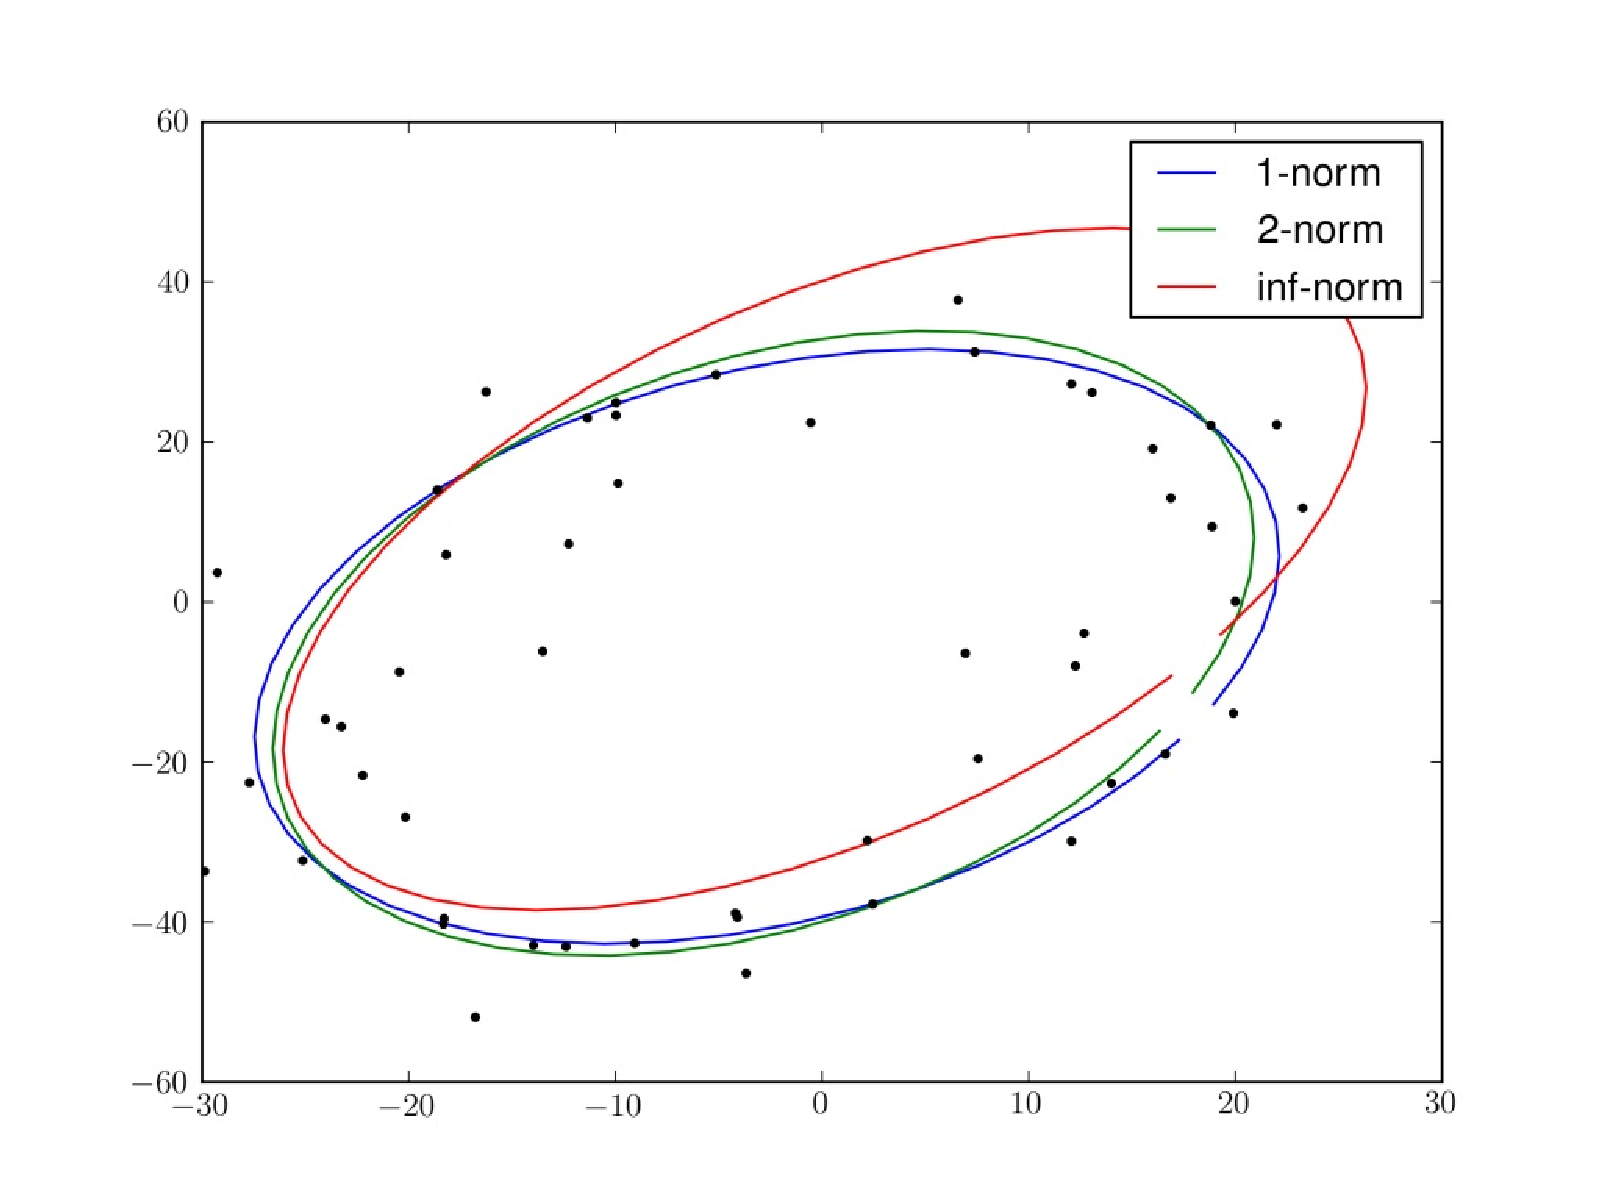
\includegraphics[width=\textwidth]{figures/ellipsefit.pdf}
\caption{Fitting an ellipse using different norms.}
\label{Fig:ellipse}
\end{figure}

\subsection*{Improvements to the QR Algorithm} % ------------------------------

\end{comment}
